\documentclass{article}

\usepackage{graphicx}
\usepackage{tikz}
\usepackage{tikzsymbols}
\usetikzlibrary{calc,patterns,shapes.geometric}
\pagestyle{empty}
\usepackage[margin=0pt]{geometry}
\geometry{papersize={14in,12in}}

\def\centerarc[#1](#2)(#3:#4:#5){\draw[#1] ($(#2)+({#5*cos(#3)},{#5*sin(#3)})$) arc (#3:#4:#5);}

\begin{document}
	\begin{figure}
		\centering
		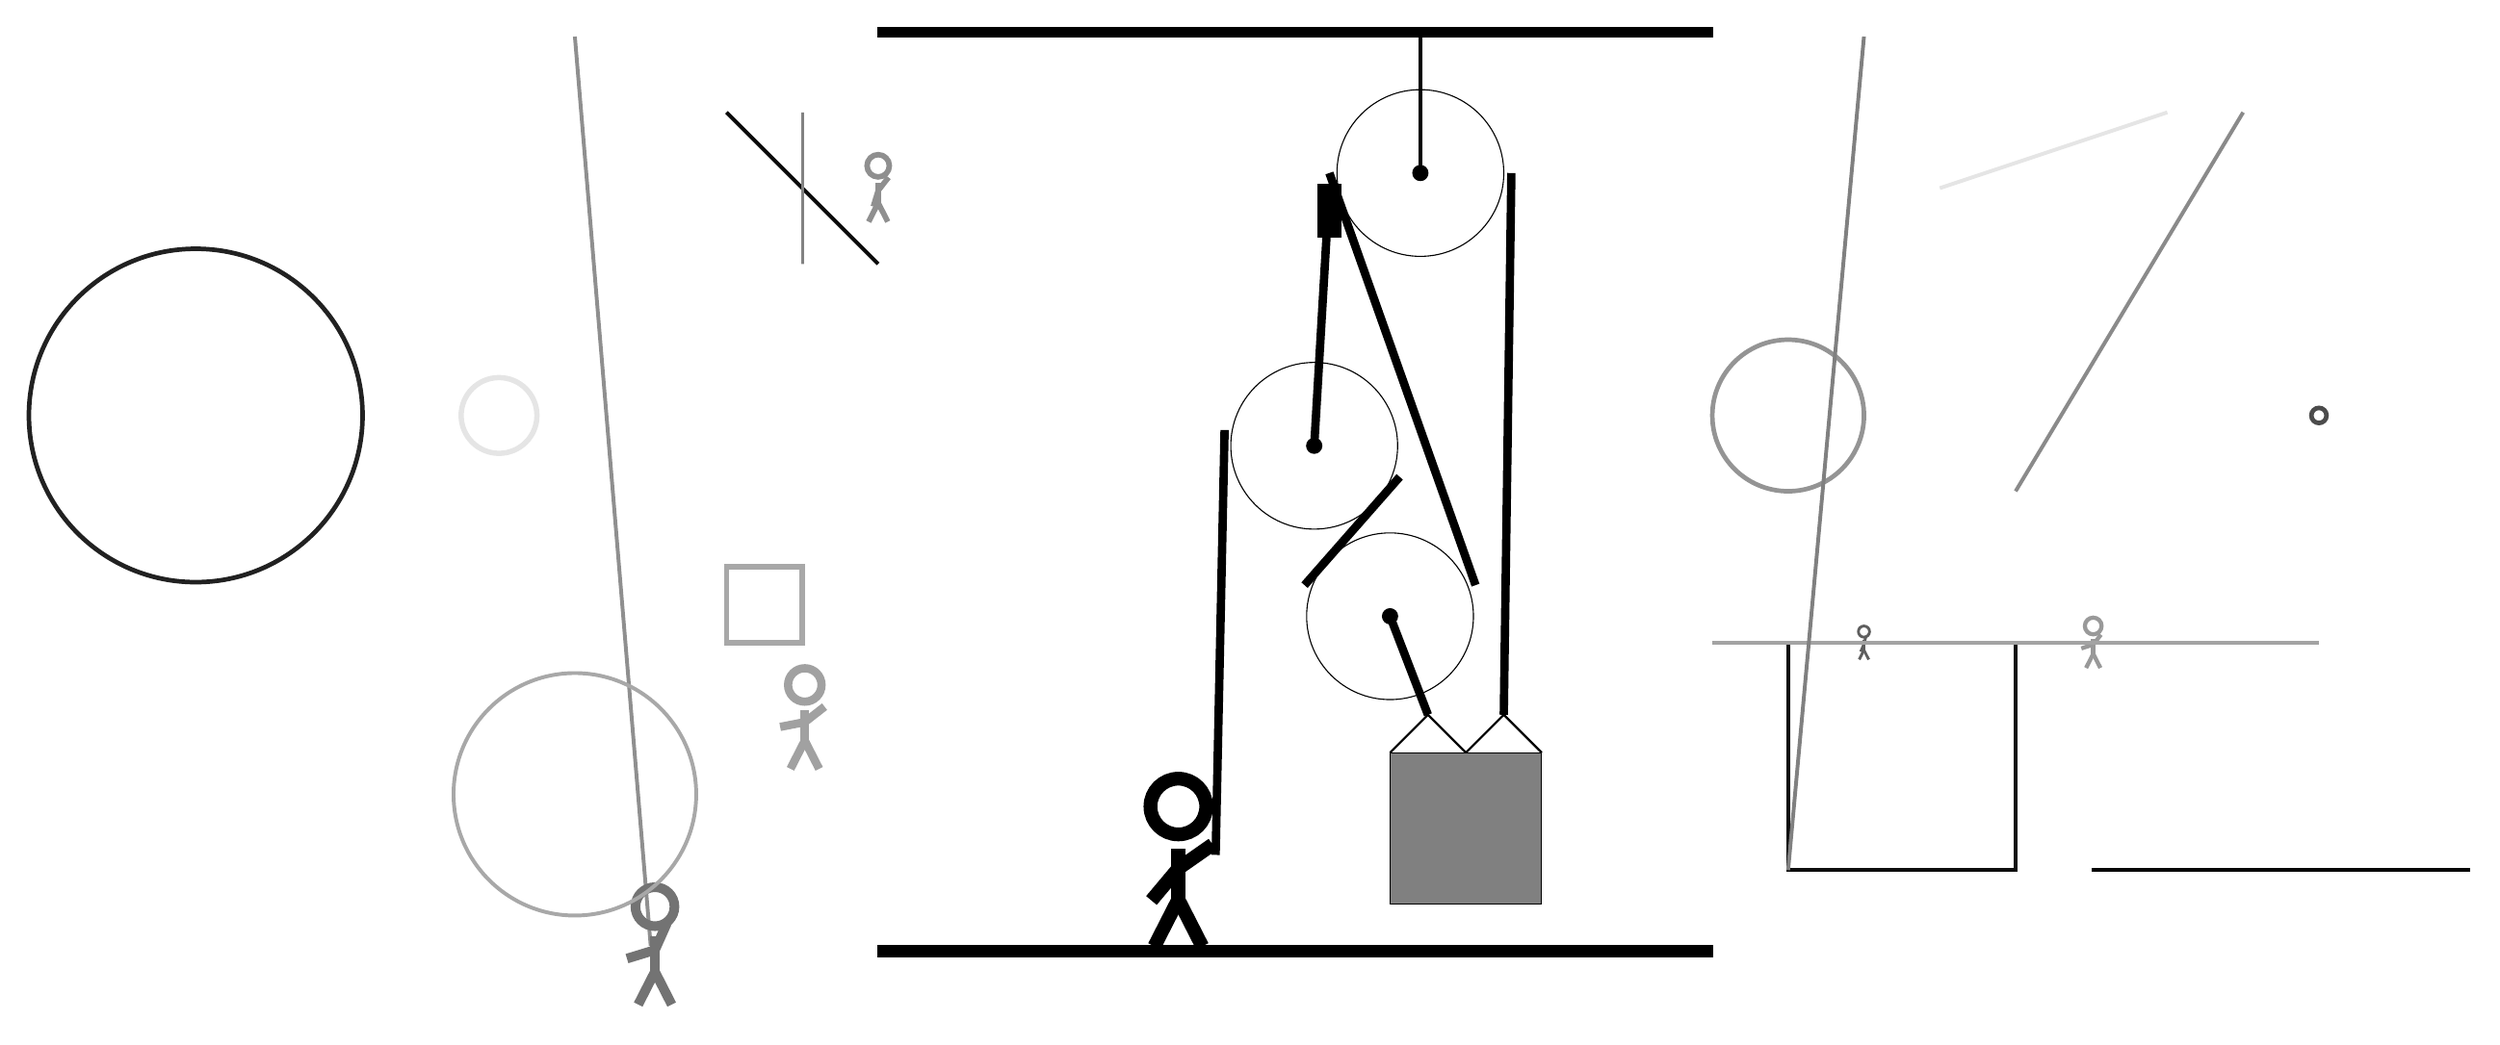
\begin{tikzpicture}
			%%%%% START %%%%%
			
			\draw[fill=black] (-6, 9) rectangle (5, 9.125);
			
			\draw (-0.25, 3.6) circle (1.1);
			\draw[fill=black] (-0.25, 3.6) circle (0.1);
			
			\draw (0.75, 1.35) circle (1.1);
			\draw[fill=black] (0.75, 1.35) circle (0.1);
			
			\draw [line width=0.5mm, color=black!67](6, 0) circle (0.0);
			
			\draw[line width=0.5mm, color=black!10](8, 7) -- (11, 8);
			\draw [line width=0.7mm, color=black!10](-11, 4) circle (0.5);
			\node[line width=0.7mm, color=black!63] at (7, 1) {\Strichmaxerl[2][67][75]};
			
			\draw[line width=0.5mm, color=black!46](9, 3) -- (12, 8);
			
			\node[line width=0.3mm, color=black!44] at (-6, 7) {\Strichmaxerl[4][73][52]};
			
			\draw [line width=0.6mm, color=black!42](6, 4) circle (1.0);
			\draw[line width=0.5mm, color=black!96](-6, 6) -- (-8, 8);
			\draw [line width=0.5mm, color=black!77](-11, 0) circle (0.0);
			\node[line width=0.6mm, color=black!37] at (-7, 0) {\Strichmaxerl[6][11][38]};
			\draw [line width=0.6mm, color=black!87](-15, 4) circle (2.2);
			\draw[line width=0.5mm, color=black!44](-10, 9) -- (-9, -3);
			\draw[line width=0.4mm, color=black!49] (-7, 6) rectangle (-7, 8);
			\draw [line width=0.6mm, color=black!70](13, 4) circle (0.1);
			\node[line width=0.2mm, color=black!40] at (10, 1) {\Strichmaxerl[3][18][52]};
			\draw[line width=0.5mm, color=black!98](10, -2) -- (15, -2);
			\node[line width=0.6mm, color=black!55] at (-9, -3) {\Strichmaxerl[7][17][66]};
			
			\draw[line width=0.7mm, color=black!34] (-8, 2) rectangle (-7, 1);
			\draw [line width=0.5mm, color=black!34](-10, -1) circle (1.6);
			\draw[line width=0.5mm, color=black!95] (6, -2) rectangle (9, 1);
			\draw[line width=0.5mm, color=black!36](5, 1) -- (13, 1);
			
			\draw[line width=0.5mm, color=black!50](6, -2) -- (7, 9);
			
			
			\draw (1.15, 7.2) circle (1.1);
			\draw[fill=black] (1.15, 7.2) circle (0.1);
			\draw[very thick] (1.15, 7.2) -- (1.15, 9);
			
			\draw[thick]  (0.75, -0.45) -- (1.25, 0.05) -- (1.75, -0.45) -- (2.25, 0.05) -- (2.75, -0.45);
			\draw[fill=black!50] (0.75, -0.45) rectangle (2.75, -2.45);
			
			\draw[line width=1.1mm] (-0.25, 3.6) -- (-0.05, 7.0);
			\draw[line width=1.1mm, fill=black](-0.15, 6.4) rectangle (0.05, 7.0);
			\draw[line width=1.1mm] (-1.55, -1.8) -- (-1.4318, 3.8083);
			\centerarc[line width=1.1mm](-0.25, 3.6)(-20:170:1.2000000000000002);
			\draw[line width=1.1mm] (0.8776, 3.1896) -- (-0.3776, 1.7604);
			\centerarc[line width=1.1mm](0.75, 1.35)(160:380:1.2000000000000002);
			\draw[line width=1.1mm] (1.8776, 1.7604) -- (-0.05, 7.2);
			\draw[line width=1.1mm](0.75, 1.35) -- (1.25, 0.05);
			\centerarc[line width=1.1mm](1.15, 7.2)(0:180:1.2000000000000002);
			\draw[line width=1.1mm] (2.35, 7.2) -- (2.25, 0.05);
			
			\node at (-2, -1.9) {\Strichmaxerl[10][50][35]};
			
			\draw[fill=black] (-6, -3) rectangle (5, -3.15);
			
			%%%%% END %%%%%
		\end{tikzpicture}
	\end{figure}	
\end{document}